% \RequirePackage{scrlfile}
% \ReplacePackage{scrpage2}{scrlayer-scrpage}
\documentclass[a4paper,twoside,12pt,chapterprefix=false]{scrbook}

\usepackage{amsmath,amssymb,amsthm}
\usepackage[footnotesize,sl,SL,hang,tight]{subfigure}  % helpful package for aligning figures next to each other
\usepackage{longtable} % tables over several pages
\usepackage[font={small,sl},hang,labelfont=bf]{caption} % configure captions
%\usepackage{captcont} % continue sufigures over several pages
\usepackage{booktabs} % publication quality tables for LaTeX
%\usepackage{showkeys} % shows the labels above the references for easier development
\usepackage{comment}
\usepackage{cleveref}

\Ifpdfoutput{%
	\usepackage[pdftex]{graphicx}
	\usepackage[]{pdfpages} %for including full pdf pages
}{%
	\usepackage{graphicx}
}
\usepackage{rotating} % rotate figures
\usepackage{placeins} % For FloatBarrier

\usepackage{scrpage2}
\KOMAoptions{headinclude}

% Font packages:
\usepackage{times}
\usepackage{helvet}   % sets sans serif font
\usepackage[T1]{fontenc}

%PDF hyperref config
\Ifpdfoutput{%
	\usepackage[pdftex,
		bookmarks,
		bookmarksopen=true,
		bookmarksnumbered=true,
		pdfauthor={My Name},
		pdftitle={Thesis Title},
		colorlinks,
		linkcolor=black,
		citecolor=black,
		filecolor=black,
		urlcolor=black,
		anchorcolor=black,
		menucolor=black,
		breaklinks=true,
		pageanchor=true,
		plainpages=false,
		pdfpagelabels=true]{hyperref}
}{}

\Ifpdfoutput{%
	\pdfcompresslevel=9
	\pdfoutput=1
	\DeclareGraphicsExtensions{.pdf,.png}
}{}

\bibliographystyle{alpha}

% Uncomment the chapter / section you are working on.
%
%\includeonly{figures}
%\includeonly{tables}
%\includeonly{data-analysis}
%\includeonly{conclusion}
%\includeonly{apx-sample-appendix}

%\pagestyle{useheadings}

% A4
%
\topmargin -0.5in
\textheight 9.3in
\textwidth 6.3in
\oddsidemargin 0.18in
\evensidemargin -0.22in
\parskip 0.1in
\parindent 0in

\renewcommand{\arraystretch}{1.5}
\renewcommand{\baselinestretch}{1}

% commands
\newcommand{\Adjoint}{\mbox{\rm Adj}}
\newcommand{\Area}{\mbox{\rm Area}}
\newcommand{\ACos}{{\mbox{\rm Cos}^{-1}}}
\newcommand{\ASin}{{\mbox{\rm Sin}^{-1}}}
\newcommand{\ATan}{{\mbox{\rm atan2}}}
\newcommand{\Code}[1]{{\tt #1}}
\newcommand{\Complex}{\mbox{\bf C}}
\newcommand{\Cross}{{\mbox{\rm Cross}}}
\newcommand{\Mydddot}[1]{\mbox{\shortstack{$.$\hspace*{-1pt}$.$\hspace*{-1pt}$.$\\$#1$}}}
\newcommand{\Degree}{\mbox{\rm degree}}
\newcommand{\Diag}{\mbox{\rm Diag}}
\newcommand{\Dim}{\mbox{\rm dim}}
\newcommand{\Dist}{\mbox{\rm Distance}}
\newcommand{\IntTwo}{\int\!\!\int}
\newcommand{\IntThree}{\int\!\!\int\! \!\int}
\newcommand{\Kernel}{\mbox{\rm kernel}}
\newcommand{\Kross}{\mbox{\rm Kross}}
\newcommand{\Grad}{\nabla}
\newcommand{\Perp}{\mbox{\rm Perp}}
\newcommand{\Point}[1]{{\cal #1}}
\newcommand{\Rank}{\mbox{\rm rank}}
\newcommand{\Range}{\mbox{\rm range}}
\newcommand{\Real}{{\mbox{\rm I}\hspace*{-2pt}\mbox{\rm R}}}
\newcommand{\RealSbt}{{\mbox{\rm\scriptsize I}\hspace*{-2pt}\mbox{\rm\scriptsize R}}}
\newcommand{\Res}{\mbox{\rm resultant}}
\newcommand{\Sbt}[1]{{\mbox{\rm\scriptsize #1}}}
\newcommand{\MySign}{\mbox{\rm Sign}}
\newcommand{\SignSBT}{\mbox{\rm\scriptsize Sign}}
\newcommand{\Skew}{\mbox{\rm Skew}}
\newcommand{\Span}{\mbox{\rm Span}}
\newcommand{\SqrDist}{\mbox{\rm Distance$^2$}}
\newcommand{\Trace}{\mbox{\rm Trace}}
\newcommand{\TRN}{{\mbox{\rm\scriptsize T}}}
\newcommand{\Vector}[1]{\mbox{\bf #1}}
\newcommand{\VectorM}[1]{\mbox{\boldmath $#1$}}
\newcommand{\Volume}{\mbox{\rm Volume}}

\newcommand{\IVec}{\mbox{\boldmath $\imath$}}
\newcommand{\JVec}{\mbox{\boldmath $\jmath$}}
\newcommand{\KVec}{\mbox{\boldmath $k$}}
\newcommand{\LVec}{\mbox{\boldmath $\ell$}}
\newcommand{\RMat}{{\cal R}}
\newcommand{\QMat}{{\cal Q}}
\newcommand{\QCMat}{\overline{\cal Q}}

\newcommand{\Lerp}{\mbox{\rm lerp}}
\newcommand{\Slerp}{\mbox{\rm slerp}}
\newcommand{\Quad}{\mbox{\rm quad}}
\newcommand{\Squad}{\mbox{\rm squad}}

\newcommand{\subsubsubsection}[1]{{\sc #1}}

\newcommand{\ODer}[2]{\frac{d #1}{d #2}}
\newcommand{\ODerT}[2]{\frac{d^2 #1}{d {#2}^2}}
\newcommand{\ODerM}[3]{\frac{d #1}{d #2 \, d #3}}
\newcommand{\PDer}[2]{\frac{\partial #1}{\partial #2}}
\newcommand{\PDerT}[2]{\frac{\partial^2 #1}{\partial {#2}^2}}
\newcommand{\PDerM}[3]{\frac{\partial^2 #1}{\partial #2 \, \partial #3}}

% mass density symbol
\newcommand{\Den}{\delta}

% environments
\newenvironment{BArray}[1]{\left\{ \begin{array}{#1}}{\end{array} \right\}}
\newenvironment{Combin}{\left( \begin{array}{c}}{\end{array} \right)}
\newenvironment{Matrix}[1]{\left[ \begin{array}{#1}}{\end{array} \right]}

% "Figure" environment
\newtheorem{localFigure}{Figure}[chapter]
\newenvironment{Figure}[1]{
  \begin{center}
  \begin{minipage}{6in}
  \par\noindent\hspace*{0pt}\hrulefill
  
  \begin{localFigure} \label{#1}
}{
  \end{localFigure}
  \par\noindent\hspace*{0pt}\hrulefill
  \end{minipage}
  \end{center}
}

% "Table" environment
\newtheorem{localTable}{Table}[chapter]
\newenvironment{Table}[1]{
  \begin{center}
  \begin{minipage}{6in}
  
  \begin{localTable} \label{#1}
}{
  \end{localTable}
  \end{minipage}
  \end{center}
}

% "CDROM" environment for source code on disk
%\newenvironment{CDROM}[1]{
%  \label{#1} 
%    \includegraphics{cdrom.png} \hspace*{0.1in}{\tt PointShop3D}. \rm
%}{
%  $\bowtie$
%}

% TO DO search symbol
\newcommand{\TODO}{\mbox{\large\bf TO DO}}
\newcommand{\REFR}{\mbox{\large\bf REFR}}

%  Terminates current page and paragraph, makes sure next page starts on
%  an odd-number, and generates a completely blank page, without page markers,
%  if necessary.
\newcommand{\clearemptydoublepage}{\newpage{\pagestyle{empty}\cleardoublepage}}

%%% Shoemake's commands
\DeclareMathOperator{\prp}{\text{\scshape perp}}
\DeclareMathOperator{\rot}{rot}
\DeclareMathOperator{\N}{N}
\providecommand{\vmag}[1]{\lVert#1\rVert}
\providecommand{\mutate}[1]{\overleftarrow{#1}}
\providecommand{\T}[1]{{#1}^{\mathrm T}}
\newcommand{\cross}{\times}
\newcommand{\by}{\times}
\newcommand{\vect}[1]{\mathbf{#1}}
\newcommand{\mat}[1]{\mathbf{#1}} % or not
%\newcommand{\quat}[1]{\mathbf{#1}}
\newcommand{\quat}[1]{\ensuremath{\mathbf{\dot{#1}}}}
\newcommand{\vV}{\vect{v}}
\newcommand{\vU}{\vect{u}}
\newcommand{\vE}{\vect{e}}
\newcommand{\vUh}{\hat{\vect{u}}}
\newcommand{\mQ}{\mat{Q}}
\newcommand{\mR}{\mat{R}}
\newcommand{\mM}{\mat{M}}
\newcommand{\mA}{\mat{A}}
\newcommand{\mB}{\mat{B}}
\newcommand{\mI}{\mat{I}}
\newcommand{\mJ}{\mat{J}}
\newcommand{\mX}{\mat{X}}
\newcommand{\mY}{\mat{Y}}
\newcommand{\mZ}{\mat{Z}}
\newcommand{\qo}{\quat{1}}
\newcommand{\qi}{\quat{i}}
\newcommand{\qj}{\quat{j}}
\newcommand{\qk}{\quat{k}}
\newcommand{\xh}{{x}}
\newcommand{\yh}{{y}}
\newcommand{\zh}{{z}}
\newcommand{\ch}{c}
\newcommand{\sh}{s}
\newcommand{\gt}{\theta}


%%
%%
%%

\setlength\parindent{0pt}
\newenvironment{TempText}{\color{gray}\normalsize}{\ignorespacesafterend}
\excludecomment{TempText}

\begin{document}

%% Define leading chapter pages
%
%\addtokomafont{chapter}{\setlength{\parskip}{190pt}}   % SEVERE HACK to keep spacing to chapter art work
\renewcommand*{\chapterheadstartvskip}{\vspace*{215pt}}  % different hack to keep spacing to chapter artwork
%\addtokomafont{chapter}{\rmfamily}        % remove this if you prefer sans-serif section titles
%\addtokomafont{section}{\rmfamily}        % remove this if you prefer sans-serif section titles
%\addtokomafont{subsection}{\rmfamily}     % remove this if you prefer sans-serif section titles
%\addtokomafont{subsubsection}{\rmfamily}  % remove this if you prefer sans-serif section titles
%\addtokomafont{paragraph}{\rmfamily}      % replace by \sffamily if you prefer sans-serif para titles
\addtokomafont{paragraph}{\sffamily}

\def\mychpstyleintl{%
{\noindent\setlength{\tabcolsep}{0pt}\setlength{\arrayrulewidth}{2pt}%
\begin{tabular}{c}
\\[100pt]
\begin{tabular}{lr}
\begin{tabular}{p{0.6\linewidth}}
\\
\end{tabular}
&
\begin{tabular}{p{0.4\linewidth}}
\rightline{{%
\sffamily%
\fontseries{bx}%
\fontshape{n}%
\fontsize{100}{120}%choose baselineskip to be 1.2 times font size
\selectfont
\thechapter}}
\end{tabular}
\end{tabular}\\[300pt]
\end{tabular}
}}
\newpagestyle{mychapterpagestyle}{{\protect\mychpstyleintl}{\protect\mychpstyleintl}}{}
\newpagestyle{myappendixpagestyle}{{\protect\mychpstyleintl}{\protect\mychpstyleintl}}{}
%%

%% macros e.g.
\newcommand{\mfytext}[0]{my fancy text}

%refs
\newcommand{\chpref}[1]{Chapter \ref{#1}}
\newcommand{\secref}[1]{Section \ref{#1}}
%\newcommand{\equref}[1]{Equation \ref{#1}} %better use builtin \eqref{}
\newcommand{\figref}[1]{Figure \ref{#1}}
\newcommand{\tabref}[1]{Table \ref{#1}}
\newcommand{\apxref}[1]{Appendix \ref{#1}}
%%

\hypersetup{pageanchor=false} % disabling anchors for title page to avoid warning

%% Replace this by your own design of a title page
%
%\title{Thesis Title}
%\author{My Name}
%\date{September 2042}
%\maketitle
%\clearemptydoublepage
% --- selfmade version ----
\begin{titlepage}
	%\topmargin 1.0cm
	\oddsidemargin 0.0cm
	\evensidemargin 0.0cm
	%\textwidth 6.5in
	
	% GameLab Logo
	\raggedleft \includegraphics*[width=0.5\textwidth]{figures/gpl_logo} \\
	
	% Titel / Slogan / Teaser
	\centering
	\Huge
	\vspace{2.0cm}
	\textbf{\textsf{SandPerSand}} \\[1.0cm]
	\large
	\textbf{\textsf{"Survival of the Fittest"}} \\[1.0cm]
	\includegraphics*[width=1.0\textwidth]{figures/teaser_temp} \\ [2.0cm]
	
	% Group Members
	\sffamily
	\raggedright
	\vfill
	
	\large
	
	
	\begin{itemize}
	    \item[Jasper --]
	     \textbf{Producer}, Programmer \\
	    \item[David --]
	     \textbf{Co-Producer} (organisatorial), Programmer, Gameplay Designer, Visual Artist, Content Creation
	     \item[Rik --] 
	     Programmer, Gameplay Designer 
	     \item[Todor --]
	     Programmer, Level Designer 
	     \item[Yuchen --]
	     Programmer, Level Designer, Visual Artist, Content Creation
	     \item[Clemens --]
	     Programmer, Level Designer, Visual Artist, Content Creation
	\end{itemize}
	
	%\vfill
	%\includegraphics*[width=0.3\textwidth]{figures/ETH_logo} \hfill
	%\includegraphics*[width=0.3\textwidth]{figures/CGL_logo}
	%\vspace{3.4cm}
\end{titlepage}
\clearemptydoublepage
%%

\hypersetup{pageanchor=true}
\pagenumbering{roman}
\setcounter{page}{1}

%\include{abstract}

%include task description here:
%\cleardoublepage
%\includegraphics[viewport=3cm 0cm 20cm 27.5cm]{task_description} %better use includepdf below!
%\includepdf{task_description}
%\cleardoublepage

%include acknowledgment here:
%\include{acknowledgment}

\tableofcontents
%\cleardoublepage
\newpage

%\addcontentsline{toc}{chapter}{List of Figures}
%\listoffigures
%\cleardoublepage

%\addcontentsline{toc}{chapter}{List of Tables}
%\listoftables
%\cleardoublepage

\pagenumbering{arabic}
\renewcommand*{\chapterpagestyle}{mychapterpagestyle}
\renewcommand*{\chapterformat}{} % show chapter titles only (no numbers)
% \setchapterpreamble[o]{...}  unfortunately does not move the \chapter output downwards

% ---- MAIN PART ----

\chapter{Formal Project Proposal}

\begin{TempText}
	(Max 10 pages)
\end{TempText}

\begin{TempText}
	@Note: Use this chapter for Rough Draft Proposal/Final Proposal 
\end{TempText}

\begin{TempText}
	@Note: A formal game proposal makes up the first chapter of your project notebook. The game proposal describes your game idea, provides a detailed development schedule, and gives a qualitative assessment of your project. The proposal should be professionally prepared, expressive, grammatically sound, illustrative of your efforts and process, and easy to understand. A good design effort can easily be hampered by a poor communication of what was done	
\end{TempText}

% ====================================================================================

\section{Game Description}

\subsection{Overview}

\begin{TempText}
	@Note: What is the genre of your game? Is it a 2D or 3D game? Is it a single player or multiplayer game? Explain the main goal of the game and/or the main purpose to be achieved by players. 
\end{TempText}

\begin{TempText}
	@Important: You need to design a project whose complexity fits the timeline of the course and the skills of your group.
\end{TempText}

\begin{TempText}
	@Important: Your game needs to really stand out in one way, but not all ways. Doing one aspect of it well will get you a better grade than doing a mediocre job on a lot of things.
\end{TempText}

We are developing a 2D, round-based, local multiplayer, semi-cooperative platformer race game. The main goal of the game is to navigate a maze-like decrepit tower structure and escape the rapidly rising mountain of quicksand piling up at the below. The game is round-based where the rounds are fast-paced bursts of cooperation, betrayal, and action. A player wins after a culmination of rounds by obtaining the highest score via escapes and collectibles overall.

A player who is too slow to climb or stands on the rising sand for a time, gets stuck in it and is engulfed. That player loses the round and joins the game again at the start of the next round.

The players are engaged in a race to the top as escaping first is the main objective of each round and gives the player the bonus of first-choice in an in-between-round item shop. While there are items to collect during the level, these have relatively minor effects/power ups/buffs compared to those which are found in the round-shop.

Each item can be used both cooperatively and/or adversarially. For example, with a ``chain-fling'' item, a player can prevent another player from reaching the top by pulling them down, or help another player by flinging them up.

Each level has a number of small built-in challenges which require one or more players to complete. They are simple to understand and quick to complete, and have a boon for completing them (e.g., items or currency). The idea being that completing a challenge requires cooperation but can also lead to betrayal by players. For example, one challenge might require a group of players to stand on a specified platform for the platform to activate and quickly move upwards. But if one player jumps off the platform during its accent, the platform breaks, leaving those who chose not to jump off to fall and recover.

\subsection{Background Story}

% \subsubsection{The Opening}
You, as players, are a group of aliens who really love shopping. This is the fantastic shopping trip to the earth that you have long been dreaming of. However, your spaceship crashed when you were entering the atmosphere. All your hard-earned money flew away from the broken window. And, instead of going to a big city, your spaceship hit in the middle of nowhere in a desert. You picked up the only dollar that happened to fall beside you, with tears rolling in your eyes.

Right at this moment, you heard some sound, it was from two archaeologists passing by, they were heading to an underground ruin. From their conversation, you knew there are full of treasures! Following them, you reached the bottom of the ruin. You stopped to stare at the face of a mummy, they didn't look completely lifeless, did they? Unfortunately, as in every mummies' story, you triggered the trap. The poor archaeologists died there. Sands are gushing out from all directions. Now, all you want to do is to grab every single treasure in your sight and head back to the ground!

Wait, what is that? Shops! It turns out there are shops run by mummies, they are alive! They don't seem to be bothered by the falling apart ruin, after all, they set those traps themselves and had fun watching stupid and greedy humans trying to survive( because they can't leave here and they are so bored). They sell powerful items to you for a more exciting escaping show, first come, first served. The passion for shopping is rekindled in your heart. You as a top shopaholic, would not stand that your buddy reaches to each mummy’s shop before you do— and rap your first chance of picking the items.

% \subsubsection{Connection to the Gameplay}



\begin{TempText}
    
    
    
	@Note: Describe any background or storyline associated with the game.
\end{TempText}

\subsection{Design Decisions}

This section goes in detail about the various important components of our game. We first describe the general structure of the game and for what purpose it is designed. After that we go over the central external force in the game, the sand, and how we plan to implement it and how we expect it to behave. We quickly note on Player Death since it is tied to the Sand. We then elaborate on he general level design and the structure of a general level in the game. Then, we go over an element of the level design, the \emph{Challenges} and their role in the player dynamic. We then describe the planned \empg{Items} for the game ad how they will function and interact with the players, as well as rudimentary inventory mechanics. We explain the purpose and function and rules regarding the \emph{end-of-round Shop}. Once this is laid out, we propose a control scheme for the game as well as the expected player state machine as well as some of the more intricate state within it.

\subsubsection{Winning Condition and Game Structure}

The game is designed to be played as a group of 2-6 players using gamepad controllers as the input method.

The game is a series of rounds where the number of rounds the game lasts is given before the game is played. Each round is played on a new/reset level.

The winning condition for any player is to have the most number of first-escapes (explained later) and/or collectibles after X rounds have passed. A first-escape occurs when a player finishes the round first.

If two players are tied in the number of first escapes, the next metric is the number of collectibles they have at that moment.

\subsubsection{Round End}
Each round ends 10 seconds after the first player reaches the goal at the top of the level. A countdown appears to indicate the time left. Players who reach the end of the level are admitted to the end of round shop.


\begin{figure}
    \centering
    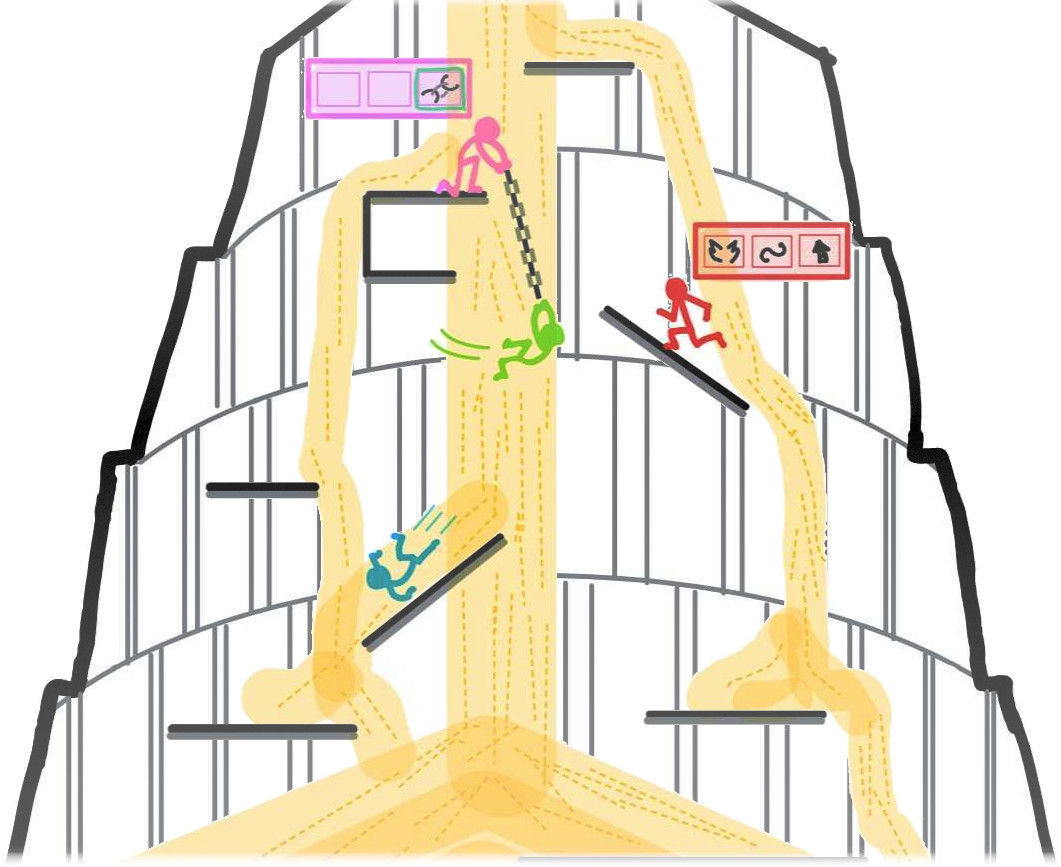
\includegraphics{figures/topmeifyoucan_concept.jpg}
    \caption{Concept of four players racing to the top with one falling due to sand, and others using an item cooperatively.}
    \label{fig:concept}
\end{figure}

\subsubsection{Sand}

The core mechanic of our game is the rising sand-mountain which acts as the main antagonistic force, swallowing players as they fall into it. 

When the rising sand catches up with a player they start sinking into it and become \emph{trapped}. In order to escape the sand, the player needs to spam the jump button (as explained in the Player State Machine). If a player falls into the sand from considerable height, or while \emph{staggered}, they get swallowed by it immediately. 

When a player dies in this way, they lose their items and a portion of their gems and gold. This forces the players to keep moving upwards and makes trying to loot the entire tower impossible, thereby putting pressure on the players when making decisions.

The sand is falling from the top of the tower, flowing along platforms and interacting with the players. This will be implemented as a separate object from the \emph{rising sand} mound itself. We project that this will be some form of a \textbf{cellular automaton} with a grid of a higher resolution than that of the overall level. This dynamically simulated sand will be player-interactable; it will push on players in the direction of flow. Player will be able to stand on this sand as it lays on platforms. Using some \emph{major items} player will be able to both create and/or destroy this kind of sand in the level during play.

\subsubsection{Player Death}
Player death can only occur when a player is trapped by the rising sand for the required duration or collides with it at high speed. Player death is temporary, a player who has died enters a countdown. After the countdown has completed, the player is respawned in the last position below the current last player

Player death erases the player's inventory, major and minor item included, and erases a percentage of collectibles they have.

Player death is recorded as a statistic.


\subsubsection{Level Design}

The game will have 2D sprite graphics inspired by architectural styles.

The levels will be on a grid with the addition of 45°, $\arctan{0.5}$ (one up, two across), and $\arctan{2}$ (two up, one across) slopes. In this grid two types of platforms will be placed. The first type can be jumped through from the bottom, the second cannot. \emph{Collectibles} will be placed all over the level to reward players for getting to an area first. These act as in-game currency and will also be spawned upon completion of \emph{Challenges}.

\subsubsection{Challenges}

The purpose of challenges is to slow players down and give them opportunities to interact and make decisions. As such they are not in themselves especially challenging, but rather a conduit for interesting social play between the players.
\par
A few challenges we will consider implementing are:

\begin{itemize}
    \item A lever which opens a door the player themselves cannot necessarily reach.
    \item Two buttons two players need to stand on to be dropped down a trap door into a room with rewards.
    \item A fast elevator which only starts when two players are inside it. If a player jumps off, it slows down significantly and traps the remaining player(s).
    \item Two buttons which starts a button mashing contest between two players standing on them. The winner gets a treasure chest dropped down to them.
\end{itemize}

\subsubsection{Items}

Items are added to the game to give the players ways to overcome obstacles, provide further opportunities for cooperation and betrayals, and to add variety to the game play. There are two types of items, but first we must describe an important input method we plan to use with the majority of items. 

\par
\textbf{Directional Selection}
\label{sec:dir-sel}
\\
Some Items (marked with a “D”) are selection directional. These items can target another player and apply effects to them, or if no player is selected when the item button is released, the item effects are applied to self (marked with an "S") or a random player (marked with an "R") depending on the item.
\par
A player with such an Item should press and hold the trigger corresponding to said item. While the trigger is held, the other trigger is disabled. The player can use the right control stick to choose another nearby player. This will be indicated via an outline of that player in the selecting player’s color as well as a line from the selecting player to the selected player in the selecting player’s color.
\par
When the player enters the selection state, the default selection is themselves. Pointing the right stick in the general direction of another player switches the selection to that player. If the stick is untouched, the default behavior for the item (self, random, or no effect) is performed.

\textbf{Picking Items Up}

If a player does not carry a minor item, and they walk over or collide with one, then they automatically pick that item up. On the other hand, once a player is carrying an item, they get the choice of swapping the item they are carrying with the item they walk over using the interact button.

The same is true for major items. When buying a major item in the end-of-round shop while one is already carried, the carried item is lost and replaced by the newly bought one.


\par
\textbf{Minor Items}
\\
A minor item can be picked up during play in the level. A player can only hold on to one minor item simultaneously. Minor power-ups should have relatively small effects and are always single use and expire at the end of the level. Minor Items act as reward during play; they are incentives to reach higher and/or solve cooperative challenges which likely require cooperation.
\par
The following is a breakdown of the minor items in the game.

\begin{itemize}
    \item Freeze Player (D/S)\\
This directional minor item freezes the selected player in place and makes them enter the trapped state. The trapped player is trapped for 7 seconds, or until they reach the trapped exit condition. If the player selects themselves, the item affects them.
    \item Control swap (R/D)\\
This random or directional item inverts the controls of a selected player, or if no player was selected, or a random player (excluding the player who activated the item). The inverted controls are indicated to the affected player via an aura around their sprite or on icon. The inversion lasts for 7 seconds.
    \item Temporary speed-up / Slow-down (D/S)\\
This directional item slows or speeds up a selected player or self. After the selection, the next input from the right stick indicates if a speed-up or slow-down is to be applied. While a player is sped up or slowed down, they retain real-time control, i.e., their inputs are not buffered or slowed. This would make certain jumps in the level easier if slowed, or make a longer jump possible. The maximum jump height of the affected player is adjusted accordingly (slightly increased or decreased, respectively). The effect lasts for 7 seconds.
    \item Double Jump (D/S)\\
A player who activates this item is granted one double jump. This is indicated to the player via an aura or an icon. They are allowed to jump once more while in the air. Once the jump is executed, the aura disappears, as does their ability to execute a double jump.
\end{itemize}

\par
\textbf{Major Items}
\\
Major items can only be obtained from the end-of-round shop. A player can only hold on to one major power-up at a time. Major items can have a large effect on the game and/or the players.
\par
The following is a breakdown of the major items in the game.

\begin{itemize}
    \item Player Position Swap (D/R)\\
The player who activates this item selects another player to swap position, and linear momentum with, essentially swapping the players. If no directional selection was carried out, a random player is selected for the swap.
    \item Rope of Binding (D)\\
A player latches themselves to another via a rope of fixed length. Thereby, the two players cannot be farther than the rope’s length from each other.
The rope does not interact with level platforms.
After a delay, either player can choose to cut the rope, indicated by the rope changing color.
A player can be suspended, hanging from the rope, and swing while in such a state.
    \item Create sand - Punch a hole in the wall\\
When a player activates this item, they punch a hole in the back wall in their current position. Sand begins to flow from that point (that grid cell and an area of cells become sand source cells). 
    \item Remove sand\\
A player can activate this item, and any sand in an area around them is destroyed. This includes source cells. This way, the player can change the flow of the game, literally.
    \item Slow Motion Time\\
When a player activates this item it globally slows down time for a duration of time.
\end{itemize}

\subsubsection{End-of-Round Shop}
At the end of each round, the players who finished the round get to access the shop. This shop will have a different selection of major items for varying prices for sale each round. The players access the shop in the same order they finished the level, so the fastest player gets first pick. However, if the first player to finish does not have enough collectibles/currency, they might not be able to buy the item they want. This detail, we feel, will encourage tactical play instead of the game being purely about getting to the top of the level fastest.

\subsubsection{Controls}

\begin{figure}
    \centering
    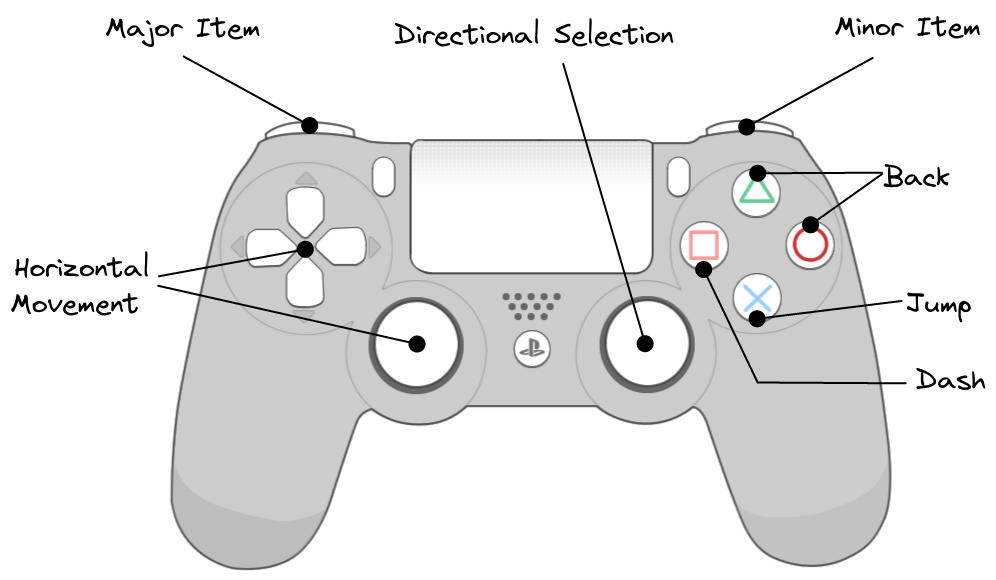
\includegraphics[width=0.8\textwidth]{figures/game_controls.png}
    \caption{Control map during play.}
    \label{fig:game_controls}
\end{figure}

\begin{figure}
    \centering
    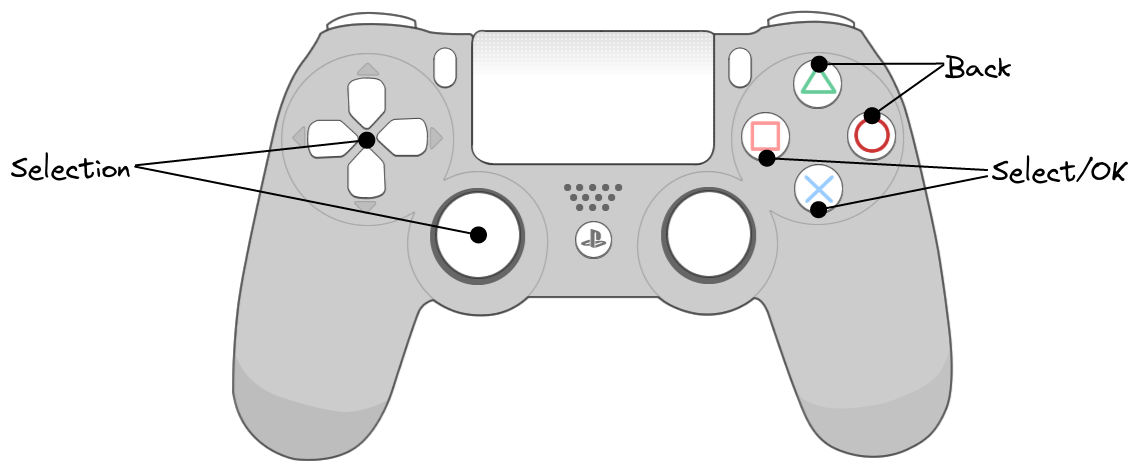
\includegraphics[width=0.93\textwidth]{figures/menu_controls.png}
    \caption{Control map for UI and Menus.}
    \label{fig:menu_controls}
\end{figure}

See the proposed control maps in Figure \ref{fig:game_controls} and Figure \ref{fig:menu_controls}.
Controls of our game follow conventions found in other platformer games. The shoulder buttons are used for the respective items (major/minor) and the right analog stick is used for directional selection (see Items section). 

\subsubsection{Player State Machine}

We expect the player state machine to have the states and state transitions shown in Figure \ref{fig:state_machine}. Of important note are the \emph{Coyote Time}, \emph{Trapped}, and \emph{Staggered} states.

A Player enters the \emph{Coyote Time} state if they run off of a platform of the platform disappears below them. In either case, the player is airborne without executing a jump. We would like to allow the player to execute a jump in this state for some number of frames, therefore being more forgiving to non-frame perfect input. This state will last 5 frames and during it the player can execute a jump as if they are grounded.

A Player enters the \emph{Trapped} state when they either stand on the rising sand for a duration or have an item which induces this state used on them. In this state, the player ceases to be able to control their movement and instead is forced to bottom mash the jump button in order to fill a meter which depletes as a constant speed, before it becomes empty. If the meter is filled quickly enough, the player exist the sate, Otherwise, when the meter runs out, the player enters the \emph{Staggered} state.

In the \emph{Staggered} state the player is unable to move or make other inputs. They are susceptible to any sand flow and will be carries with greater speed than usual by it. The state lasts for a duration. If a player touches the rising sand while in this state, they instantly are submerged and die, and wait to be respawned. 


\begin{figure}
    \centering
    \includegraphics[width=0.8\textwidth]{figures/state_diag.png}
    \caption{Player State Machine diagram.}
    \label{fig:state_machine}
\end{figure}


\begin{figure}[h]
    \centering
    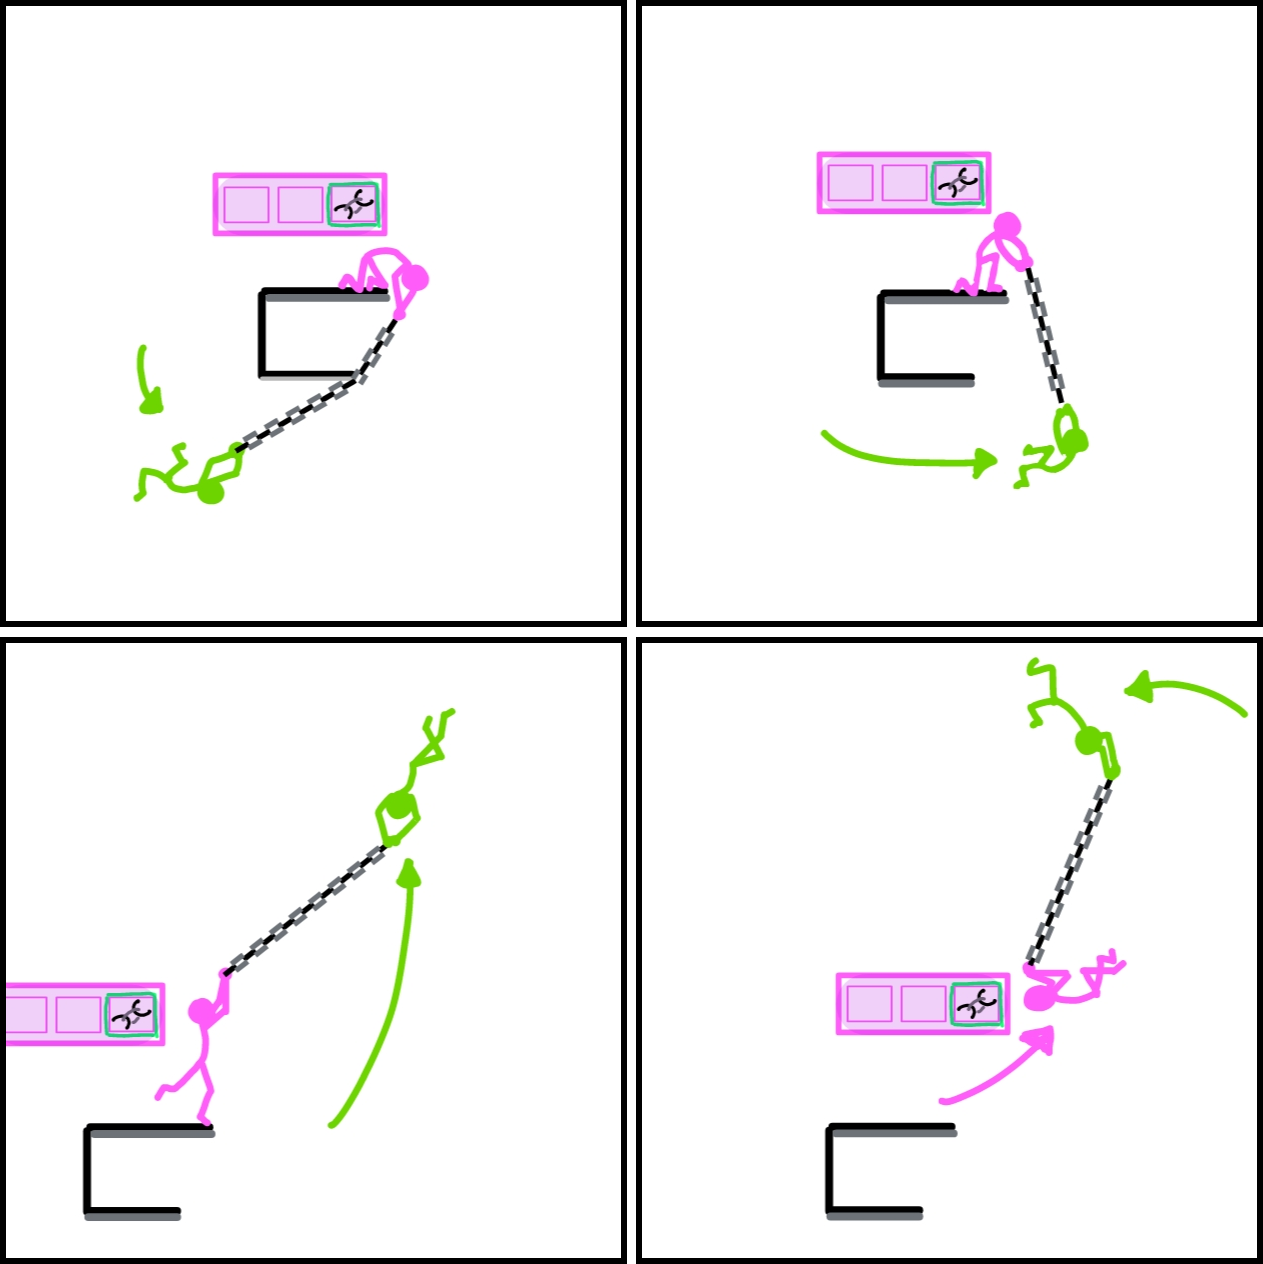
\includegraphics[width=0.5\textwidth]{figures/topmeifyoucan_concept_rope_coop.png}
    \caption{Concept of two players using an item cooperatively.}
    \label{fig:concept-coop}
\end{figure}

\begin{figure}[h]
    \centering
    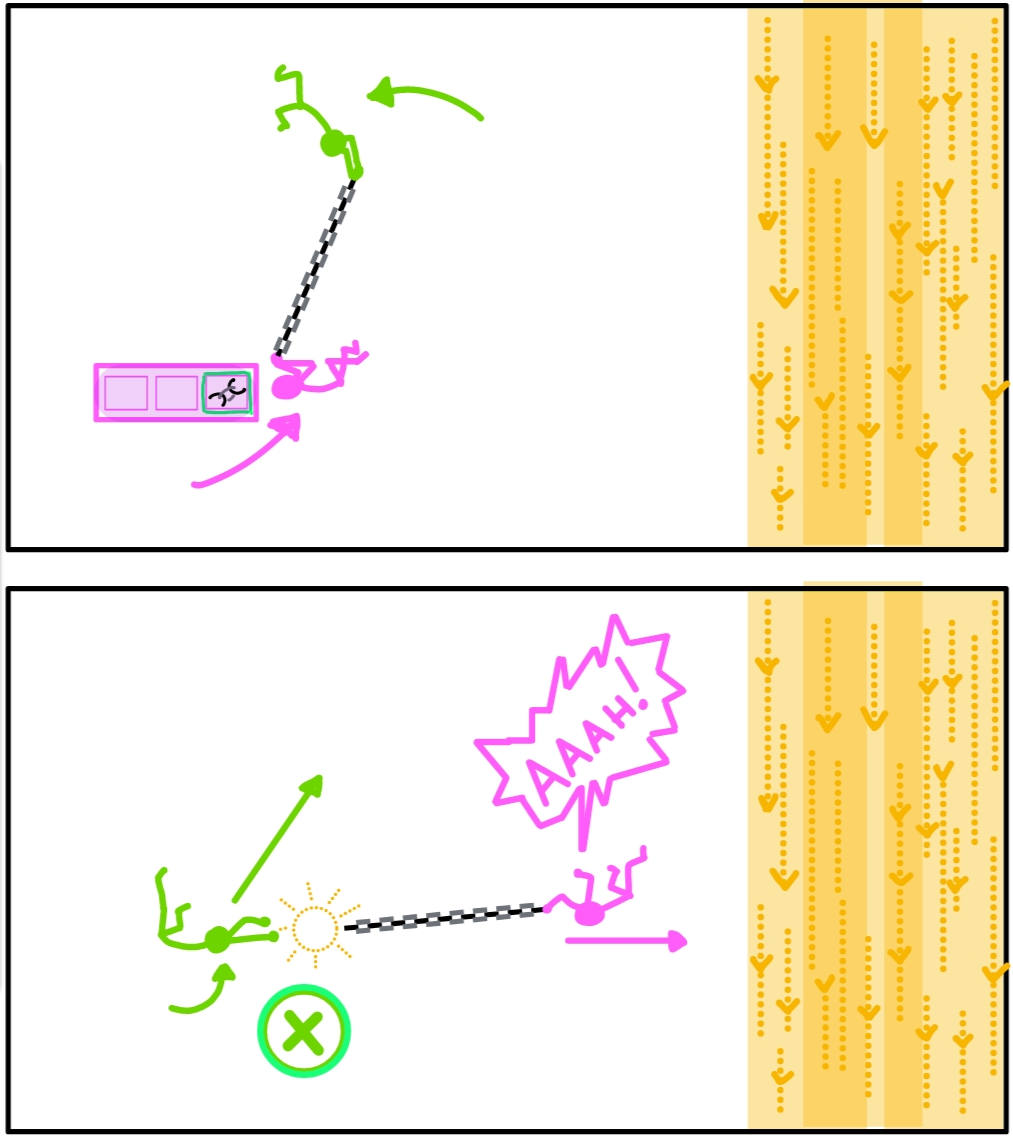
\includegraphics[width=0.5\textwidth]{figures/topmeifyoucan_concept_rope_betrayal.png}
    \caption{Concept of a player using an item adversarially. One player releases the chain to fling the other into a downward sand stream.}
    \label{fig:concept-betrayal}
\end{figure}

% ====================================================================================

\section{"Big Idea" Bullseye}

\begin{TempText}
	@Note: Highlight the primary, central, most important conceptual idea of your game, as well as the central, supporting, extra-special and impressive technical component. Your entire team should agree upon and buy into these two concepts during the design phase so that everything that goes into the project is focused and aligned around a common and unified goal. It sounds a bit obvious, but it's a powerful tool.
\end{TempText}

\begin{TempText}
	@Note: Include a graphic big idea bullseye in your game proposal. The primary and secondary drives should be short, direct, and to the point.
\end{TempText}

The bullseye of our game is the social aspect we are trying to achieve. The game will give tools for the player to cooperate and play against one another while ultimately only allowing one winner. Therefore we are expecting alliances of varying durations to from during the game only to be broken at the latest by the end of the game.
\par
The technical components facilitating this will be mini challenges strewn throughout the levels which require multiple players to overcome, but provide ample opportunities for betrayal, as well as the collection of small items and power ups and the input-control design.

% ====================================================================================

\section{Technical Achievement}

\begin{TempText}
	@Note: Your game should include at least one core technical item. This technical element should help your game stand out in an innovative way by providing an element that goes beyond the normal functionalities. This is your chance to select a concept from another course or something that you have always been interested in and implement it in the context of your game. Try to impress us, while still ensuring that the concepts you target fit within the scope of the course.
\end{TempText}

\begin{TempText}
	@Note: This section should detail the core technical item you plan to include. You are free to present more than one idea, but remember that it's better to be super successful at one item than to try to include many and fail.
\end{TempText}

We plan on the technical achievement of our game to be a Dynamic Sand Simulation. Since the sand plays such a central role in our game design and ties our game to the theme, we will make sure this feature stands out as a technically impressive and well-polished feature of the game. We believe this is an appropriate challenge and that there are several ways we could choose to implement this which proves a sliding scale as to how challenging we want it to be.

% ====================================================================================

\section{Development Schedule}

\begin{TempText}
	@Note: The development schedule is crucial and should contain two basic parts. First, you must provide a layered development description of your game that divides the development schedule into five categories based on how crucial each element is. Second, you must provide a timeline for the course including major milestones and deliverables.
\end{TempText}

\begin{TempText}
	@Note: Structure your development so that you complete each layer before going on to the next. Plan exactly what is entailed in each layer, and which team member is going to do each component. Include this layered description in your proposal.
\end{TempText}

\subsection{Layered Task Breakdown}

\begin{TempText}
	@Note: You can't accurately anticipate how long each step in your project is going to take. Consequently, you need to make a detailed development schedule that is layered.
\end{TempText}

The following list presents the different targets that our team aims to achieve, and gives a short description of what each of them contains. We are still in the process of breaking some of these down into concrete work packets.

\subsubsection{Functional Minimum}

\begin{TempText}
	@Note: Minimal items to make something that you might call a game. You'd be embarrassed if you only got this far, but at least it'd be something.
\end{TempText}

The functional minimum is a single-player platforming experience. It includes at least one level where the player jumps from platform to platform. The controls and the collision detection need to be implemented.

\subsubsection{Low Target}

\begin{TempText}
	@Note: Your target for what you want to get done--the least possible to feel sort-of OK about the result.
\end{TempText}

The low target is a local multiplayer game, which uses gamepads. The game is expected to be played by a group of friends at a party, so the rounds will be kept up to at most 4-5 minutes long.
    
The aim of the players is to race to the top of the level, while sand is rising from the bottom. Touching the sand kills the players. The first player to reach the top wins the round.
    
Unlike the functional minimum, the players will be animated. This will improve the visual aesthetic of the game and make it more appealing.

\subsubsection{Desired Target}

\begin{TempText}
	@Note: This is what you're aiming for, if things go reasonably well.
\end{TempText}

In addition to winning the round, the desired target will include conditions to win the game overall. This can be the conclusion of the overarching story of the game, with the winner being clearly shown and congratulated for their achievement by a win screen.

The game will involve buying of items between rounds. Those items will be bought by players with money that will be collected during the level and at the end of each round based on the order in which they finish. Those items can be used to more easily win subsequent rounds, such as speed boosts, power boosts and so on.

The game will additional have small challenges in the rounds. Those challenges would involve a simple puzzle that may require the collaboration of more than one players. Those challenges will not be mandatory to complete the round, but will give the player additional coins or items.

\subsubsection{High Target}

\begin{TempText}
	@Note: It might be possible to get this much done, if all goes extremely well.
\end{TempText}

The high target will further include breakable sand platforms, which will break after a given set of seconds upon standing on them.

Each round will begin with a starting challenge, that needs to be completed by all players in collaboration before the sand starts rising and the timed part of the game commences.

Additionally, a ranking for the players and statistics for each round will be shown in the end.

The shop will further include additional items to buy.

\subsubsection{Extras}

\begin{TempText}
	@Note: Stuff that you know you can't get done this semester, but you might add later if you decide your game is cool enough to keep working on after the class is over, just for fun.
\end{TempText}

Additional rubber banding for the weakest players, so that they continue playing and having fun.

Additionally, sand will be falling from the top to the bottom throughout the levels, which will interact with the player and slow them down or kill them.

A player can trap another player via the cage item. The player can stay close to the cage they have dropped in order to make it last longer.

A binding mechanic which allows players to attach to each other and help with the completion of the levels. The players can choose to detach themselves from each other after a given period of time has passed.

Mini boss fights inside the rounds, in which the players are forced to collaborate in order to succeed.

Items can hit the players while they race to the top, which slows them down or kill them.

\subsection{Task List}

% draw art assets, 
% animation,
% level design,
% audio,
% player control,
% game engine,

% \begin{itemize}
%     \item 12.03.2022
%     \begin{enumerate}
%         \item Report chapter 1 - Project proposal (Final formal version)
        
%         6 people - All
%     \end{enumerate}
    
%     \item 19.03.2022
%     \begin{enumerate}
%         \item Report chapter 2 - Prototype
        
%         4 People - Todor, Yuchen, Clemens and David
%         \item Game Engine
        
%         2 People - Jasper and Rik
%     \end{enumerate}
    
%     \item 26.03.2022
%     \begin{enumerate}
%         \item Game release 1 - First playable demo (Minimum Target)
%         \item One level
        
%         2 People - Yuchen, Clemens
        
%         \item Controls
        
%         2 Person - David, Todor
        
%         \item Improving the Game Engine
        
%         2 People - Jasper, Rik
%     \end{enumerate}
    
%     \item 02.04.2022
%     \begin{enumerate}
%         \item Sand
        
%         3 People - Jasper, Todor, David
%         \item Local Multiplayer
        
%         3 People - Yuchen, Rik, Clemens
%     \end{enumerate}
    
%     \item 09.04.2022
%     \begin{enumerate}
%         \item Sand
        
%         3 People - Jasper, Todor, David
%         \item Winning Condition
        
%         3 People - Rik, Yuchen, Clemens
%     \end{enumerate}
    
%     \item 16.04.2022
%     \begin{enumerate}
%         \item Sound
        
%         1 Person - David
%         \item GUI
        
%         2 People - Yuchen, Clemens
%         \item Optimising everything and QA testing
        
%         3 People - Todor, Jasper, Rik
%     \end{enumerate}
    
%     \item 23.04.2022
%     \begin{enumerate}
%         \item Report chapter 3 - Interim report.
        
%         3 People - David, Clemens, Yuchen
%         \item Game release 2 - Interim demos (Low Target)
        
%         3 People - Jasper, Todor, Rik
%     \end{enumerate}
    
%     \item 30.04.2022
%     \begin{enumerate}
%         \item Items on the level to be picked up (Coins)
        
%         2 Person - Todor, David
        
%         \item Simple Shop
        
%         2 People - Rik, Yuchen
        
%         \item Challenge
        
%         2 People - Jasper, Clemens
%     \end{enumerate}
    
%     \item 07.05.2022
%     \begin{enumerate}
%         \item Report chapter 4 - Alpha release.
        
%         3 People - David, Clemens, Yuchen
%         \item Game release 3 - Alpha demo (Desired Target)
        
%         3 People - Jasper, Todor, Rik
%     \end{enumerate}
    
   
    
%     \item 14.05.2022
%     \begin{enumerate}
%         \item Report chapter 5 - Playtest.
        
%         3 People - David, Clemens, Yuchen
%         \item Game release 4 - Final version for Gobo
        
%         3 People - Jasper, Todor, Rik
%     \end{enumerate}
    
%     \item 21.05.2022
%     \begin{enumerate}
%         \item Feature Freeze / Improvements / QA
%     \end{enumerate}
    
%     \item 28.05.2022
%     \begin{enumerate}
%         \item Game release 5 - Version for final presentation (Things from High Target)
%     \end{enumerate}
    
%     \item 04.06.2022
%     \begin{enumerate}
%         \item Report chapter 6 - Conclusion.
        
%         2 People - David, ???
%         \item Demo Video
        
%         4 People - Rik, Todor, ???, ???
%     \end{enumerate}
    
%     % \item 11.06.2022
    
%     % \item 18.06.2022
    
% \end{itemize}
\begingroup
\small
\begin{tabular}{|l|l|l|l|} 
\hline
Task                                                          & start date & due date & Responsibility  \\ 
\hline
Report chapter 1 - Project proposal (Final formal version)    & 5.3.22     & 12.3.22  & all             \\
Report chapter 2 - Prototype                                  & 12.3.22    & 19.3.22  & T, Y, C, D      \\
Game Engine                                                   & 12.3.22    & 19.3.22  & J,R             \\
Game release 1 - First playable demo (Minimum Target)         & 19.3.22    & 26.3.22  & all             \\
One level                                                     & 19.3.22    & 26.3.22  & Y,C             \\
Controls                                                      & 19.3.22    & 26.3.22  & D,T             \\
Improving the Game Engine                                     & 19.3.22    & 26.3.22  & J,R             \\
Sand                                                          & 26.3.22    & 2.4.22   & J,T,D           \\
Local Multiplayer                                             & 26.3.22    & 2.4.22   & Y,R,C           \\
Sand 2                                                        & 2.4.22     & 9.4.22   & J,T,D           \\
Winning Condition                                             & 2.4.22     & 9.4.22   & Y,R,C           \\
Sound                                                         & 9.4.22     & 16.4.22  & D               \\
GUI                                                           & 9.4.22     & 16.4.22  & Y,C             \\
Optimising everything and QA testing                          & 9.4.22     & 16.4.22  & T,D,J           \\
Report chapter 3 - Interim report.                            & 16.4.22    & 23.4.22  & D,C,Y           \\
Game release 2 - Interim demos (Low Target)                   & 16.4.22    & 23.4.22  & J,T,R           \\
Items on the level to be picked up (Coins)                    & 23.4.22    & 30.4.22  & T,D             \\
Simple Shop                                                   & 23.4.22    & 30.4.22  & R,Y             \\
Challenge                                                     & 23.4.22    & 30.4.22  & J,C             \\
Report chapter 4 - Alpha release.                             & 30.4.22    & 7.5.22   & D,C,Y           \\
Game release 3 - Alpha demo (Desired Target)                  & 30.4.22    & 7.5.22   & J,T,R           \\
Report chapter 5 - Playtest                                   & 7.5.22     & 14.5.22  & D,C,Y           \\
Game release 4 - Final version for Gobo                       & 7.5.22     & 14.5.22  & J,T,R           \\
Feature Freeze / Improvements / QA                            & 14.5.22    & 21.5.22  & -               \\
Game release 5 - Version for final presentation (High Target) & 21.5.22    & 28.5.22  & -               \\
Report chapter 6 - Conclusion                                 & 28.5.22    & 4.6.22   & D               \\
Demo Video                                                    & 28.5.22    & 4.6.22   & R,T             \\
\hline
\end{tabular}
\endgroup

\subsection{Timeline}

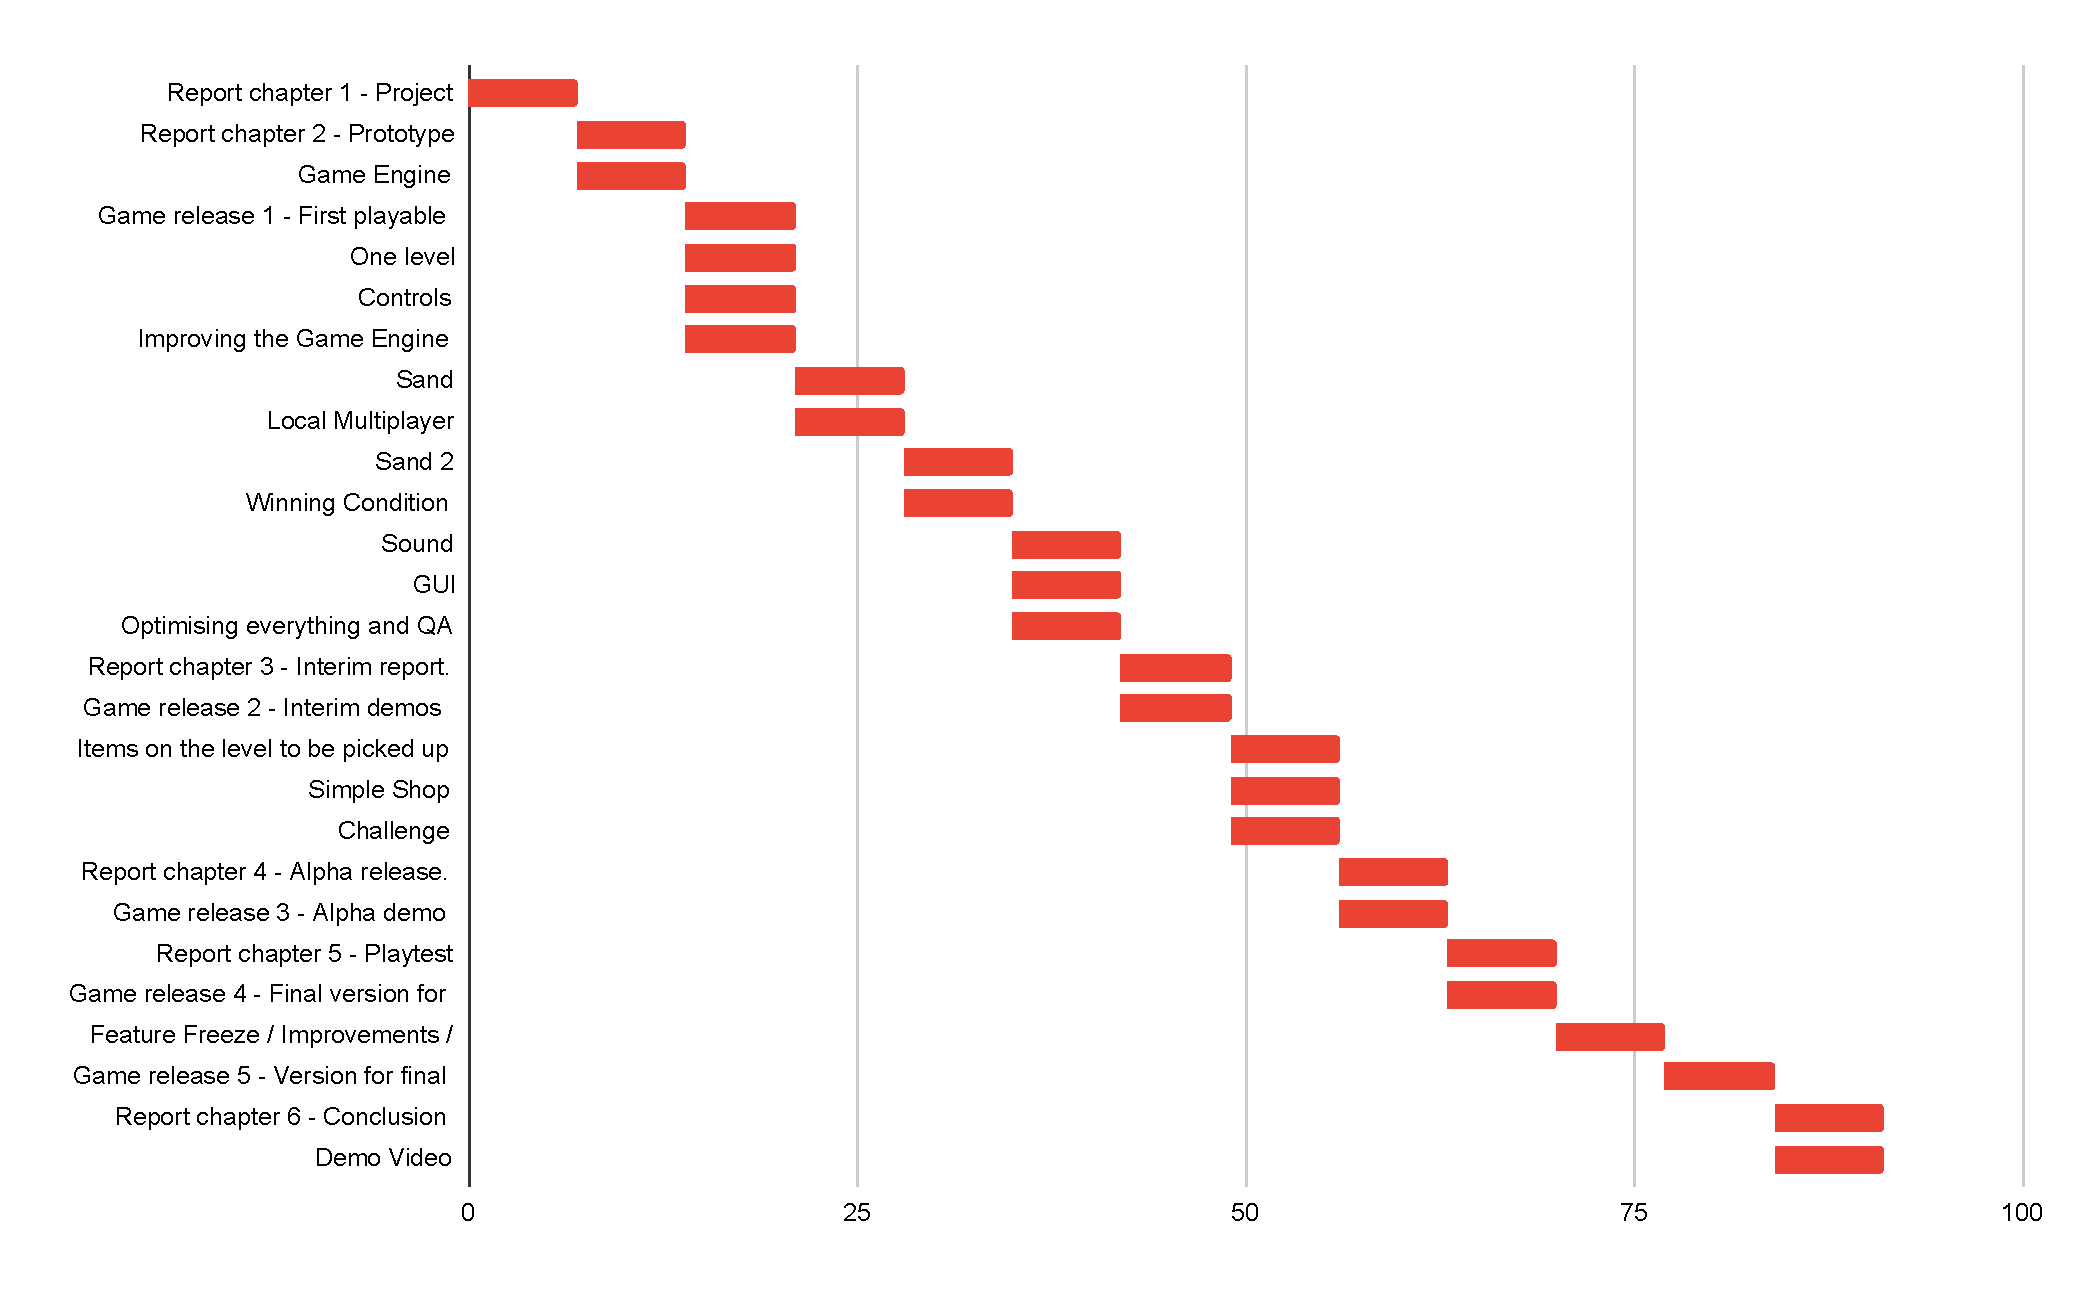
\includegraphics[width=\textwidth]{figures/GANTT_chart.pdf}

% ====================================================================================

\section{Assessment}



\begin{TempText}
	@Note: Tell us what the main strength of the game will be. What part is going to be the coolest? Who might want to play this game? What do they do in the game? What virtual world should the system simulate? Basically, you are setting up a world view for your subsequent design. What criteria should be used to judge if your design is a success or not?
\end{TempText}

\subsection{Fun-factor}
The main fun-factor of our game is the unpredictability of each round. the forming and breaking
of alliances will keep the players on the edge of their seats as they scramble to reach the top.
While the platforming action is the main appeal, the game also provides abundant opportunities
for planning. “Do I just rush past these coins and get ahead, or spend time collecting then for
a better item which will help me later in the game?” Of course, other players can and will put
and end to your plans which adds depth to the concept.


\subsection{Feasibility}
Our planned game is quite ambitious and we believe that we can make this work.

There are many interconnected parts, such as the platforms, sand, items, challenges and the shop.
In addition to that, we need to balance the individual parts to reach a state where the players actually need to consider cooperation vs. betrayal.

On the other hand, we limit ourselves to a 2D game which reduces the required effort considerably.
There are many libraries available for MonoGame that solve or simplify certain aspects of our game.
And most importantly, our team consists of motivated members with a wide variety of relevant experience, ranging from game programming to art design and sounds.
Some members already helped producing games or worked on their own game.


\chapter{Prototype}

\begin{TempText}
	(Min 3, Max 5 pages)
\end{TempText}

\begin{TempText}
	@Note: The key goal of this part of the project is to develop a prototype of your game that distills out the core game play. The prototype should incorporate the game mechanics while providing only a crude approximation of other features like artwork.
\end{TempText}

% ====================================================================================

\section{Prototype Setup}

\begin{TempText}
	@Note: Include sketches and photos of your prototype in such a way that you can demonstrate how the prototype works and how the gameplay is modeled. How did you model environment, characters, and other features of the game?
\end{TempText}

We designed a playable paper prototype \ref{fig:prot_stalll} and \ref{fig:prot_0}.

\begin{figure}
    \centering
    \includegraphics[width=0.8\textwidth]{figures/Prototype/staaall.jpg}
    \caption{In the middle of a heated race.}
    \label{fig:prot_stalll}
\end{figure}

\begin{figure}
    \centering
    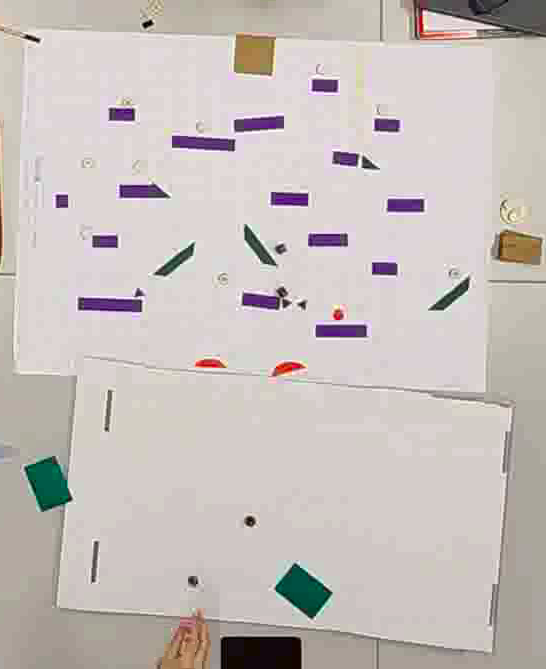
\includegraphics[width=0.8\textwidth]{figures/Prototype/vlcsnap-2022-03-20-18h52m10s352.png}
    \caption{Paper Prototype of the Game.}
    \label{fig:prot_0}
\end{figure}

\begin{figure}
    \centering
    \includegraphics[width=0.8\textwidth]{figures/Prototype/circle.png}
    \caption{Game Master determining if a move is legal}
    \label{fig:prot_1}
\end{figure}
Our design involves two types of people:
\begin{enumerate}
    \item Players: Play the game. Try to win by reaching the top first.
    \item Game Master: Controls the automated game mechanics (such as the rising sand from the bottom) and makes sure the players abide by its rules.
\end{enumerate}

The players move on a grid plane. They take rounds, in each of which they can make a move. The raising sand from the bottom is modelled by a big piece of cardboard, which is moved 4 squares up every 2 rounds. If a player touches the rising sand, he dies.

On each round the players can move/jump to a new position.
There are two type of jump:
\begin{itemize}
    \item Easy Jump: A jump that does not go through falling sand and which finishes on a platform wider than 2 squares
    \item Hard Jump: A jump that goes through falling sand or which finishes on a platform narrower than 3 squares.
\end{itemize}

The players begin at the bottom of the level. Each player is represented by a differently coloured tetrahedron.

At every round, the players have 5 seconds to choose where they want to jump. They state their intended place of movement by putting a dice on their desired location. They can also state if they intend on using an action card. The list of action cards is shown at \ref{fig:prot_1} and \ref{fig:prot_2}.



\begin{figure}
    \centering
    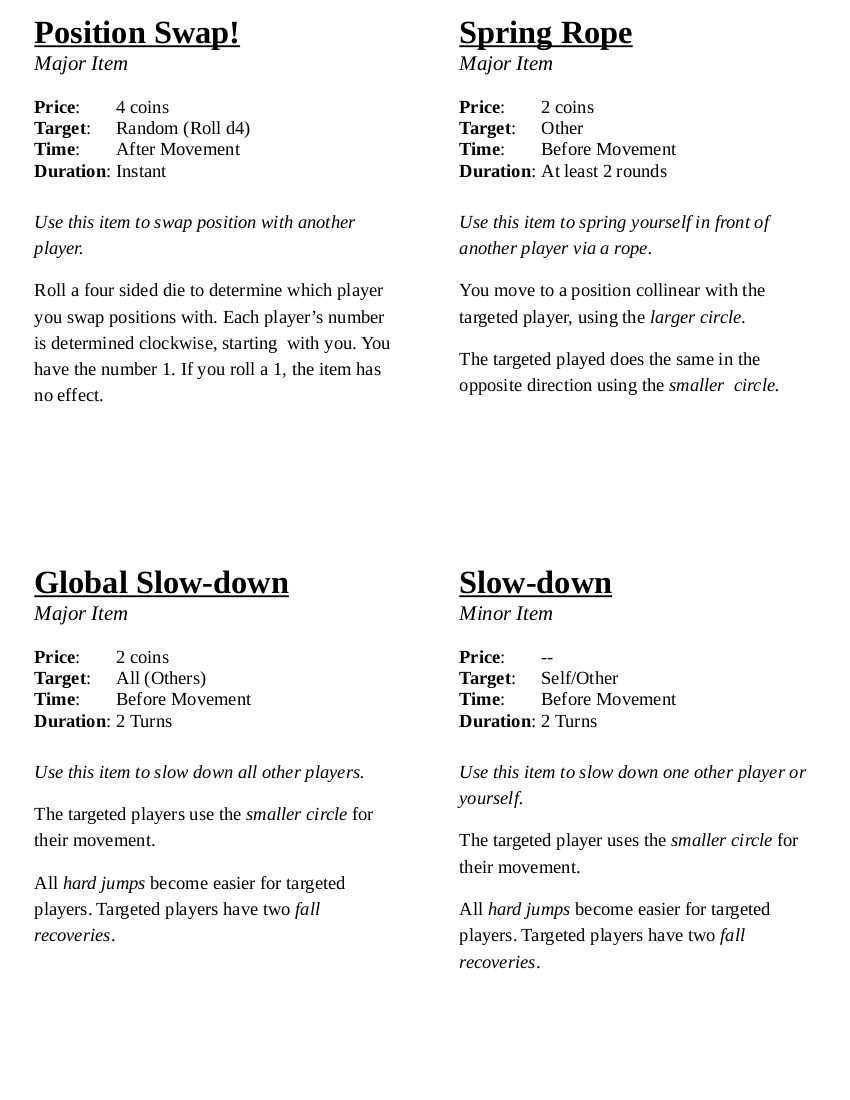
\includegraphics[width=0.8\textwidth]{figures/Prototype/topmeifyoucan_1.png}
    \caption{Action Cards.}
    \label{fig:prot_1}
\end{figure}



\begin{figure}
    \centering
    \includegraphics[width=0.8\textwidth]{figures/Prototype/topmeifyoucan_2.png}
    \caption{Action Cards.}
    \label{fig:prot_2}
\end{figure}


After the players finish making their choice, the Game Master checks if all of the movements could be performed. This is done by picking up a circle, and checking if there is a position of the circle for which the beginning and ending positions of the players are  both points on the circle, and the arc of the circle do not go through any platforms. If this is the case, then the jump is possible. If the player performs a hard jump, he must say "even" or "odd" and then roll a dice. If he correctly calls the result, he successfully makes the jump. If he fails, then the player misses the platform and starts falling. For every platform he passes while falling, he has a chance of recovery. In order for him to recover, he must correctly call "odd" or "even" on a dice. If he calls correctly, then he makes a successful recovery and lands on the platform. Otherwise he continues falling. The falling stops when he reaches the bottom of the level, or when he hits the sand, which makes him die.

The game concludes when at least two of the players reach the top (represented by a brown square  at the top of the level).


\FloatBarrier


% ====================================================================================

\section{Playing Experience}

\begin{TempText}
	@Note: Your experience playing the game. Was it fun?
\end{TempText}

We played the game for more than two hours and find it to be quite fun. We found that it is very dependant on the rolling of the dice, and therefore on luck. This is a problem that will be less of an issue with the final product, as there this "luck" aspect will be replaced by the players' skill and ability to do good jumps.

% ====================================================================================

\section{Findings and Conclusion}

\begin{TempText}
	@Note: Explain what you have learned from creating the prototype. What has proved to be harder (or easier) than expected? What design revisions have you made to your game based on your experience creating the prototype?
\end{TempText}

\begin{itemize}
    \item We confirmed that this unbounded cooperation-competition gameplay 
    works well. 
    \item Most of our designed items work well and do add uncertainties to the race.
    \item Current cooperative challenges didn't reach high usage in the prototype. We plan to refine on this part.
    
    \item We came to the conclusion that having a normal rope with which to tie two players is unnecessary. This is because it gives the players no clear advantage.

    This is the reason why the rope was modified to a "Spring Rope". Instead of tying two players together for a given set of rounds, the "Spring Rope" can be used by a player to quickly move in a given direction, similar to long jump. This makes the mechanics simpler and the item is more usable.
\end{itemize}




\chapter{Interim Report}

\begin{TempText}
	(Max 5 pages)
\end{TempText}

% ====================================================================================

\section{Progress}

\begin{TempText}
	@Note: Describe how many layers you have finished. You can include screen shots to help explain your game so far, and text to describe how a user would interact with it. Our hope is that you have completely finished layer 2 and are well into layer 3.
\end{TempText}

% ====================================================================================

\section{Challenges}

\begin{TempText}
	@Note: Explain what has proved to be harder (or easier) than expected. What design revisions have you made to your game as a result of what you've learned with the implementation? Discuss the implementation challenges you faced. Were there aspects that you wanted to build but were unable to do so?
\end{TempText}

% ====================================================================================

\section{Future Work}

\begin{TempText}
	@Note: What are the planned tasks that will be implemented next? Shortly explain.
\end{TempText}


\chapter{Alpha Release}

\begin{TempText}
	(Max 5 pages)
\end{TempText}

\begin{TempText}
	@Note: Follows the same guidelines as the interim report chapter
\end{TempText}

% ====================================================================================

\section{Progress}

\begin{TempText}
	@Note: Comment on how far you have progressed and show us what is exciting about your game. Ideally, you will have met the goals outlined in layer 3 (your desired target) and possibly part or all of layer 4 (your high target). You can include screenshots.
\end{TempText}

% ====================================================================================

\section{Challenges}

\begin{TempText}
	@Note: Explain what has proved to be harder (or easier) than expected. What design revisions have you made to your game as a result of what you've learned with the implementation? Discuss the implementation challenges you faced. Were there aspects that you wanted to build but were unable to do so?
\end{TempText}

% ====================================================================================

\section{Future Work}

\begin{TempText}
	@Note: What are the planned tasks that will be implemented next? Shortly explain.
\end{TempText}


\chapter{Playtest}

\begin{TempText}
	(Max 5 pages)
\end{TempText}

% ====================================================================================

\section{Playtesting Session}

\begin{TempText}
	@Note: Describe who you recruited for playtesting and how you organized the playtesting sessions. If possible, include some photos.
\end{TempText}

% ====================================================================================

\section{Questions and Comments}

\begin{TempText}
	@Note: List the questions you chose to ask the testers. Summarize their answers. Comment on overall trends you learned from the exercise, as well as any specific suggestions that were particularly useful.
\end{TempText}

% ====================================================================================

\section{Design Revisions}

\begin{TempText}
	@Note: Finally, describe any changes you made to your game based on the playtesting.
\end{TempText}


\chapter{Conclusion}

\begin{TempText}
	(Max 5 pages)
\end{TempText}

% ====================================================================================

\section{Final Results}

\begin{TempText}
	@Note: In this chapter, first provide a summary of your final results including screenshots from your final game. Comment on any significant changes from the alpha release.
\end{TempText}

% ====================================================================================

\section{Experience}

\begin{TempText}
	@Note: Here you should provide commentary about your experience during the class. How well did your initial design ideas materialize into the final game. Were you able to follow your development schedule, or did you deviate significantly from it? How did the different elements of the project structure (development schedule, prototype, playtesting, etc.) contribute to or hinder your progress?
\end{TempText}

% ====================================================================================

\section{Personal Impressions}

\begin{TempText}
	@Note: Did it meet your expectations? Are you happy and proud of your game? Do you feel there wasn't enough time or that the schedule was too compressed?
\end{TempText}

\begin{TempText}
	@Note:  You might also consider these questions:
	\begin{itemize}
		\item What was the biggest technical difficulty during the project? \\
		\item What was your impression of working with the theme? \\
		\item Do you think the theme enhanced your game, or would you have been happier with total freedom? \\
		\item What would you do differently in your next game project? \\
		\item What was your greatest success during the project? \\
		\item Are you happy with the final result of your project? \\ 
		\item Do you consider the project a success? \\
		\item To what extend did you meet your project plan and milestones (not at all, partly, mostly, or always)? \\
		\item What improvements would you suggest for the course organization? (Perhaps in D1 evaluation)? \\
		\item Did you like using MonoGame?
	\end{itemize}
\end{TempText}




% ---- END MAIN PART ----


%\appendix
%\clearpage
%\renewcommand*{\chapterpagestyle}{myappendixpagestyle}

%\include{apx-sample-appendix}

%\clearpage
%\renewcommand*{\chapterpagestyle}{empty}

%\nocite{*}
%\addcontentsline{toc}{chapter}{Bibliography}
%\bibliography{graphics}

\end{document}
